 \section{Evaluation}
 \label{sec:eval}

%  \wajih{the word DISTDET is not consistent in the paper.}

 %\wajih{Use macros for common words in this whole section.}

 %\wajih{Be consistent with the terminology that you used in the abstract/intro.}

 %\wajih{Captions need to be lowercase}

 {\renewcommand{\arraystretch}{1.2}
 \begin{table*}[!t]
   \centering
   \small
   \caption{Comparison of \Sys against \flash and \kairos. Prec.: Precision; Rec.: Recall; \flash has slightly better performance than our system, but \Sys preserves user privacy and achieves high scalability through decentralization, unlike \flash and \kairos.}
   \setlength{\tabcolsep}{0.7pt}
   \begin{tabular}{ccccccccccccc}
     \toprule
 
   \multirow{2}{*}{\textbf{Datasets}}
   & \multicolumn{4}{c }{\Norothead{ \bf \Sys}}
   & \multicolumn{4}{c }{\Norothead{ \bf \flash~\cite{flash2024}}}
   & \multicolumn{4}{c }{\Norothead{ \bf \kairos~\cite{cheng2023kairos}}}
   \\ \cmidrule(r{\tbspace}){2-5} \cmidrule(r{\tbspace}){6-9} \cmidrule(r{\tbspace}){10-13}
 
     & {\bf Prec.} &  {\bf Rec.} & {\bf \fscore} & {\bf TP}/ {\bf FP}/ {\bf FN}/ {\bf TN} & {\bf Prec.}  & {\bf Rec.} & {\bf \fscore} & {\bf TP}/ {\bf FP}/ {\bf FN}/ {\bf TN} & {\bf Prec.}  & {\bf Rec.} & {\bf \fscore} & {\bf TP}/ {\bf FP}/ {\bf FN}/ {\bf TN} \\
 
   \midrule
 
   E3-CADETS &  \TCP & \TCR & \TCF & \TCTP/ \TCFP/ \TCFN/ \TCTN &  \FCP & \FCR & \FCF & \FCTP/ \FCFP/ \FCFN/ \FCTN & \KCP & \KCR & \KCF & \KCTP/ \KCFP/ \KCFN/ \KCTN \\
   E3-TRACE &  \TTP & \TTR & \TTF & \TTTP/ \TTFP/ \TTFN/ \TTTN  & \FTP & \FTR & \FTF & \FTTP/ \FTFP/ \FTFN/ \FTTN & - & - & - & - \\
   E3-THEIA &  \TTHP & \TTHR & \TTHF & \TTHTP/ \TTHFP/ \TTHFN/ \TTHTN & \FTHP & \FTHR & \FTHF & \FTHTP/ \FTHFP/ \FTHFN/ \FTHTN & \KTHP & \KTHR & \KTHF & \KTHTP/ \KTHFP/ \KTHFN/ \KTHTN \\  
   \optc & \TOP & \TOR & \TOF & \TOTP/ \TOFP/ \TOFN/ \TOTN & \FOP & \FOR & \FOF & \FOTP/ \FOFP/ \FOFN/ \FOTN & \KOP & \KOR & \KOF & \KOTP/ \KOFP/ \KOFN/ \KOTN \\
   E5-CADETS &  \ETCP & \ETCR & \ETCF & \ETCTP/ \ETCFP/ \ETCFN/ \ETCTN  & \EKCP & \EKCR & \EKCF & \EKCTP/ \EKCFP/ \EKCFN/ \EKCTN & \EFCP & \EFCR & \EFCF & \EFCTP/ \EFCFP/ \EFCFN/ \EFCTN \\
   E5-THEIA &  \ETTHP & \ETTHR & \ETTHF & \ETTHTP/ \ETTHFP/ \ETTHFN/ \ETTHTN & \EKTHP & \EKTHR & \EKTHF & \EKTHTP/ \EKTHFP/ \EKTHFN/ \EKTHTN & \EFTHP & \EFTHR & \EFTHF & \EFTHTP/ \EFTHFP/ \EFTHFN/ \EFTHTN \\
   E5-ClearScope & \ETClP & \ETClR & \ETClF & \ETClTP/ \ETClFP/ \ETClFN/ \ETClTN  & \EKClP & \EKClR & \EKClF & \EKClTP/ \EKClFP/ \EKClFN/ \EKClTN & \EFClP & \EFClR & \EFClF & \EFClTP/ \EFClFP/ \EFClFN/ \EFClTN \\
   \bottomrule
   \end{tabular}
 \label{summary:benchmarks:large}
 \end{table*}}



%We evaluate \Sys using the open-source datasets \darpa E3 and \optc, which comprise system audit logs that simulate enterprise environments. These logs are collected from both Windows and Linux operating systems.

Our evaluation experiments are conducted on a machine running Ubuntu 18.04.6 LTS, equipped with a 10-core Intel CPU, NVIDIA RTX 2080 GPU, and 120 GB of memory. In our experiments, we set the federated learning rounds and the number of categorized \gnnshort to 10 per host. Each model is trained for 20 epochs per round. We use regularization and dropout layers in our models to avoid overfitting. To evaluate \Sys, we address the following research questions:

\begin{itemize}[leftmargin=*]
\item \textbf{RQ1.} How does \Sys compares to existing systems in terms of detection performance?
\item \textbf{RQ2.} How effective is the categorization based \gnnshort ensemble compared to a single \gnnshort? 
\item \textbf{RQ3.} What is the effectiveness of word2vec harmonization in a utility server setting?
\item \textbf{RQ4.} What is the resource consumption of various components of \Sys? 
\item \textbf{RQ5.} What is the end to end processing time of \Sys on a client machine? 
\item \textbf{RQ6.} How does the operational cost metrics of \Sys compares to centralized systems?

\end{itemize}

%\wajih {Say here that we have an ablation study on metrics: Effect of Federated Averaging Round, blah blah in Appendix.}

We also present a detailed ablation study in Appendix~\ref{app:ablation} on metrics, such as the effect of the number of hosts, number of \gnnshort submodels, number of federated averaging rounds, and the anomaly threshold on the detection performance.

\PP{Implementation} \Sys is developed in Python with around 5500 lines of code. It leverages the PyTorch and Torch Geometric libraries to implement the federated provenance graph learning framework. For developing the semantic attribute encoder, we employ the Gensim library. Secure communication between clients and the utility server is ensured through Python's Cryptography module. The federated averaging, semantic vector harmonization, and entity categorization modules are implemented as individual Python functions on the central and utility servers.


\PP{Datasets} We have utilized the \darpa E3~\cite{error3}, E5~\cite{bug5}, and \optc~\cite{darpaoptc} datasets for our evaluation. The E3 and E5 datasets consist of several adversarial engagements that simulate real-world APTs on enterprise networks. In these exercises, the red team aims to exploit vulnerabilities in the enterprise's services while hiding their attacks behind benign system activities. The logs captured from these exercises are documented under various scenario names, including Cadets, Trace, Theia and ClearScope. The \optc dataset, another open-source resource from \darpa, encompasses a comprehensive collection of audit logs from an enterprise environment with 1,000 hosts. This dataset includes six days of benign system logs, serving as training data for our system to learn normal behavior patterns. Subsequently, attack logs span three days of system activities, featuring red team tactics such as initial compromises, privilege escalations, malicious software installations, and data exfiltration. Each of these datasets is accompanied by ground truth documents that facilitate the distinction between benign and malicious events. For our evaluation, we employ attack labels from existing systems, such as \threatrace, \kairos and \flash for our evaluation. We evaluate our system using the same subset of datasets as existing open-source systems such as \kairos and \flash, and we utilize the attack node labels provided by them to ensure fairness.


%\wajih{Add citations. Say a few lines about the PIDS that we do not compare against. Read Kairos evaluation section -- they have very good sentences about why they don't compare against several existing PIDS. Make sure that you do not miss any PIDS system. Make sure to cite this paper: https://www.usenix.org/system/files/sec23winter-prepub-490-jia.pdf}

\PP{Detectors for comparison} To benchmark our system, we conduct comparisons against existing state-of-the-art PIDS. \threatrace~\cite{wang2022threatrace}, a node-level system, employs graph representation learning to identify anomalous nodes within a provenance graph. In contrast, \flash~\cite{flash2024}, another node-level system, outperforms \threatrace in both detection efficiency and effectiveness by leveraging semantic feature vectors and an embedding database. Given \flash's superiority over \threatrace, our comparison primarily focuses on \flash. Additionally, we include \kairos~\cite{cheng2023kairos} in our comparison, which utilizes temporal graph networks to capture the evolution of a system's provenance graph over time. We do not compare against Streamspot~\cite{streamspot} and Unicorn~\cite{han2020unicorn} as they are graph-level detectors, and recent systems like \threatrace and \flash have been shown to surpass them in detection performance. While \disdet~\cite{dong2023distdet}, Prographer~\cite{yangprographer} and Shadewatcher~\cite{shadewatcher} are notable PIDS, we exclude them from our comparison because \disdet, Prographer is closed-source and a major component of Shadewatcher is proprietary, which hinders our ability to conduct a thorough comparison. It is important to note that, similar to existing works, such as \kairos, Shadewatcher, and Prographer, \Sys considers only three node types in provenance graphs: process, files, and sockets. However, in the E3 dataset, \flash has also been evaluated using additional node types. Therefore, we executed \flash using these three node types to report the results in Table~\ref{summary:benchmarks:large}. 

 \subsection{Detection performance}
 We conducted experiments to assess how \Sys compares with other systems in terms of detection performance. Initially, we outline our methodology for deploying \Sys on the \darpa E3, E5, and \optc datasets. The E3 dataset comprises various scenarios, including Cadets, Theia, and Trace, each representing logs generated by a single host machine. To evaluate \Sys on E3, we treat each scenario as an individual host. Consequently, in our federated learning approach, we trained local \gnnshort models on each scenario individually. These local models then participated in federated averaging, a process repeated across 10 rounds. Upon completing the training, we evaluated the global \gnnshort model against the attack logs from these E3 scenarios. Similar to E3, the E5 dataset is also divided into different scenarios; however, each scenario comprises three different hosts. For each scenario, we use benign logs data from these different hosts to train our system and then evaluate it on the attack logs. For the \optc dataset, we sampled hosts for inclusion in our federated provenance graph learning experiment. Additionally, we also conducted experiments with a varying number of randomly selected hosts, the results of which are detailed in our ablation study. For conducting these evaluations, we use the same detection metrics as defined by existing node-level detectors such as \threatrace and \flash.

 Table~\ref{summary:benchmarks:large} reveals that \Sys's performance on these datasets is comparable to that of \flash, despite the data heterogeneity, diverse log patterns, and data imbalance contained within each E3, E5, and \optc clients. This underscores \Sys's capability to maintain robust detection performance amidst such heterogeneity. \kairos's evaluation, based on a coarser time-window granularity compared to the node-level granularity of \flash and \Sys, poses a challenge for direct comparison. Nevertheless, our results remain competitive with \kairos. Beyond detection performance, we also highlight \Sys's qualitative advantages, including its privacy-preserving features and decentralized, scalable operation. These aspects underscore the value of \Sys in contrast to centralized systems, emphasizing its high practicality in real-world deployments. Since \kairos was not originally evaluated on the DARPA E3 Trace, we did not compare \kairos on this dataset for fairness because unlike \flash extensive hyperparameter tuning might be needed for \kairos to produce the best results.

\subsection{Effectiveness of categorized graph learning}

To examine the effectiveness of our process categorization based \gnnshort ensemble technique, we conducted experiments comparing our ensemble technique against a single model approach in a federated setting. Specifically, for the ensemble method, we designated the number of categories to be 10. This approach standardizes all processes across various hosts into 10 distinct categories, ensuring that the \gnnshort models learn similar distributions regardless of the host. Such standardization is crucial for mitigating the impact of heterogeneous distributions and data imbalance during the federated averaging process. Table~\ref{categorized_gnn} reports the average results for the \darpa E3, E5 and \optc datasets. The results indicate that utilizing categorized ensemble models yields superior performance. This improvement is attributed to each sub-model's enhanced ability to concentrate on different patterns of system activity from different clients, thereby reducing the likelihood of these patterns becoming conflated during the federated averaging process. %\wajih{Explain the reason that why you ignored E5 here. This is a simple way a reviewer can kill your paper as you are trying to hide information.}

% \begin{table}[!t]
%   \centering
%   \small
%   \setlength{\tabcolsep}{10pt}
%   \caption{Effectiveness of categorized \gnnshort learning.}
%   \begin{tabular}{ | c | c | c | c | c |}
%     \hline
%     \bf Dataset & \bf Type & \bf Prec. & \bf Rec. & \bf \fscore \\
%     \hline
%     \multirow{2}{*}{E3-Cadets} & Single & \STCP & \STCR & \STCF \\ 
%     \cline{2-5} 
%     & Ensemble & \TCP & \TCR & \TCF \\
%     \hline
%     \multirow{2}{*}{E3-Trace} & Single & \STTP & \STTR & \STTF \\
%     \cline{2-5} 
%     & Ensemble & \TTP & \TTR & \TTF \\
%     \hline
%     \multirow{2}{*}{E3-Theia} & Single & \STTHP & \STTHR & \STTHF \\
%     \cline{2-5} 
%     & Ensemble & \TTHP & \TTHR & \TTHF \\
%     \hline
%     \multirow{2}{*}{\optc} & Single & \STOP & \STOR & \STOF \\
%     \cline{2-5} 
%     & Ensemble & \TOP & \TOR & \TOF \\
%     \hline
%   \end{tabular}
%   \label{categorized_gnn}
% \end{table}

\begin{table}[!t]
  \centering
  \small
  \setlength{\tabcolsep}{10pt}
  \caption{Effectiveness of categorized \gnnshort learning.}
  \begin{tabular}{ | c | c | c | c | c |}
    \hline
    \bf Dataset & \bf Type & \bf Prec. & \bf Rec. & \bf \fscore \\
    \hline
    \multirow{2}{*}{\optc} & Single & \STOP & \STOR & \STOF \\
    \cline{2-5} 
    & Ensemble & \TOP & \TOR & \TOF \\
    \hline
    \multirow{2}{*}{E3} & Single & 0.89 & 0.99 & 0.94 \\ 
    \cline{2-5} 
    & Ensemble & 0.96 & 0.99 & 0.97 \\
    \hline
    \multirow{2}{*}{E5} & Single & 0.92 & 0.96 & 0.94 \\ 
    \cline{2-5} 
    & Ensemble & 0.99 & 0.96 & 0.97 \\
    \hline
  \end{tabular}
  \label{categorized_gnn}
\end{table}

 \subsection{Efficacy of \wordvec harmonization}

 We evaluated the effectiveness of our \wordvec vector harmonization scheme through two experiments using the \optc, E3 and E5 datasets. In the first experiment, each client utilized its locally trained \wordvec model to encode semantic features during the training process. In the second experiment, we harmonized the individually trained models into a central \wordvec model using the utility server architecture, as explained in Section~\ref{sec:methodology}. Then each client used this centralized model for generating semantic features. Table~\ref{local:wordvec} presents the average results for the \darpa E3, E5 and \optc datasets. By employing the harmonized models, we achieved significantly better detection outcomes. This is because these local models encode different information for identical tokens across hosts. Such variability leads to heterogeneity in the feature space for the \gnnshort model, impairing the model's ability to generalize and converge effectively during the federated learning process, thereby yielding suboptimal results. However, through our novel, privacy-preserving aggregation of these semantic models, we have addressed this issue by merging the information in these models together to give the \gnnshort more generalized input vectors. %\wajih{Explain the reason that why you ignored E5 here. This is a simple way a reviewer can kill your paper as you are trying to hide information.}

%  \begin{table}[!t]
%   \centering
%   \small
%   \setlength{\tabcolsep}{9pt}
%   \caption{Effectiveness of \wordvec vectors harmonization. \mati{Getting results.}}
%   \begin{tabular}{ | c | c | c | c | c |}
%     \hline
%     \bf Dataset & \bf Type & \bf Prec. & \bf Rec. & \bf \fscore \\
%     \hline
%     \multirow{2}{*}{E3-Cadets} & Local & \ETLWCP & \ETLWCR & \ETLWCF \\
%     \cline{2-5} 
%     & Harmonized & \TCP & \TCR & \TCF \\
%     \hline
%     \multirow{2}{*}{E3-Trace} & Local & \ETLWTHP & \ETLWTHR & \ETLWTHF \\
%     \cline{2-5} 
%     & Harmonized & \TTP & \TTR & \TTF \\
%     \hline
%     \multirow{2}{*}{E3-Theia} & Local & \ETLWClP & \ETLWClR & \ETLWClF \\
%     \cline{2-5} 
%     & Harmonized &  \TTHP & \TTHR & \TTHF \\
%     \hline
%     \multirow{2}{*}{\optc} & Local & \VFOP & \VFOR & \VFOF \\ 
%     \cline{2-5} 
%     & Harmonized & \TOP & \TOR & \TOF \\
%     \hline
%   \end{tabular}
%   \label{local:wordvec}
% \end{table}

\begin{table}[!t]
  \centering
  \small
  \setlength{\tabcolsep}{9pt}
  \caption{Effectiveness of \wordvec vectors harmonization.}
  \begin{tabular}{ | c | c | c | c | c |}
    \hline
    \bf Dataset & \bf Type & \bf Prec. & \bf Rec. & \bf \fscore \\
    \hline
    \multirow{2}{*}{\optc} & Local & \VFOP & \VFOR & \VFOF \\ 
    \cline{2-5} 
    & Harmonized & \TOP & \TOR & \TOF \\
    \hline
    \multirow{2}{*}{E3} & Local & 0.83 & 0.96 & 0.89 \\ 
    \cline{2-5} 
    & Harmonized & 0.96 & 0.99 & 0.97 \\
    \hline
    \multirow{2}{*}{E5} & Local & 0.81 & 0.94 & 0.87 \\ 
    \cline{2-5} 
    & Harmonized & 0.99 & 0.96 & 0.97 \\
    \hline
  \end{tabular}
  \label{local:wordvec}
\end{table}

 \subsection{Resource consumption}

 We conducted experiments to analyze the resource consumption of the central, utility server, and client-side modules of \Sys. We modeled the resource utilization on a client machine using different batches of audit events of varying sizes. For the central and utility servers, we studied resource consumption by varying the number of clients to understand the demands of federated averaging and semantic vector harmonization. The results, depicted in Figure~\ref{fig:resource}, indicate that \Sys's resource consumption is moderate. Specifically, \Sys can process up to 100,000 audit events simultaneously while consuming less than 900 MB of memory and utilizing less than 20\% of CPU resources. This performance suggests that \Sys does not significantly burden the client machine, especially considering the typically low event throughput on such machines. Consequently, our system only needs to execute a few times per day to process newly accumulated events, indicating that resource consumption is not continuous but intermittent. Additionally, our analysis of the host data in the \optc dataset shows that, on average, each client generates approximately 100,000 audit log events within a three-hour period. For the central and utility servers, the resource usage is minimal, demonstrating that our architecture is scalable and suitable for large organizations with many clients.

 \begin{figure}[!t]
  \centering
  \subfloat[CPU utilization client side.]{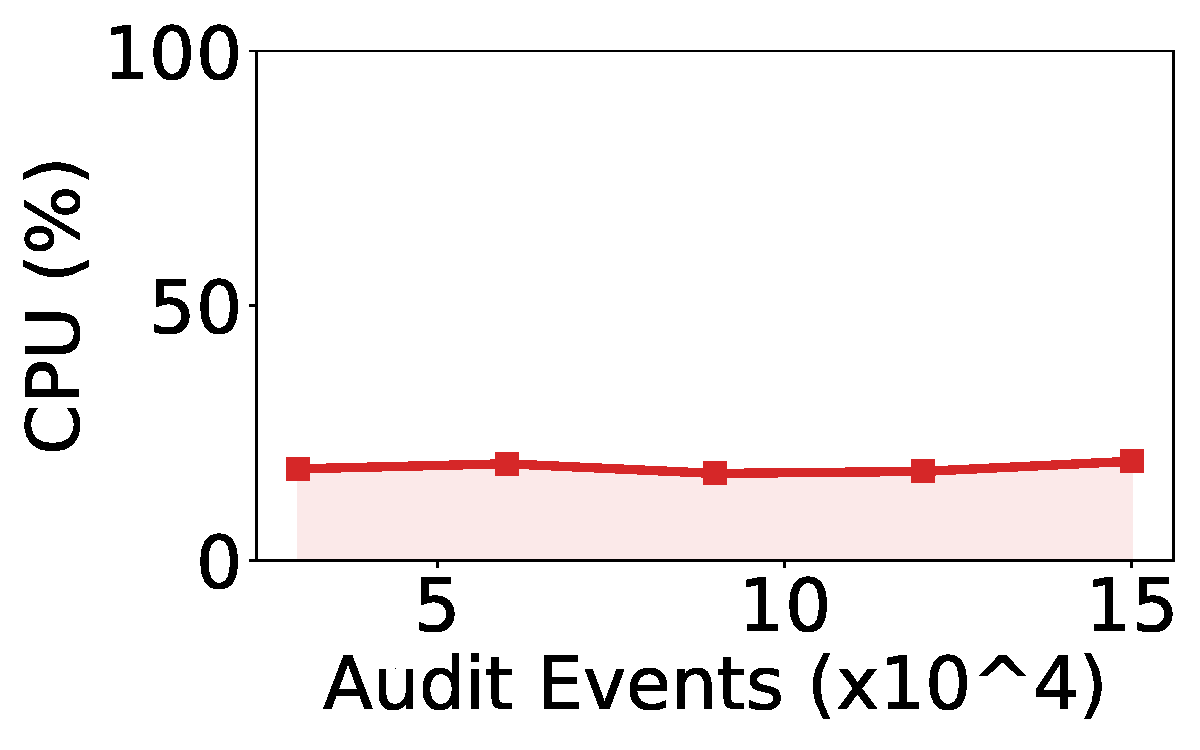
\includegraphics[width=0.20\textwidth]{fig/cpu.pdf}\label{cpu_client}}
  \hfill
  \subfloat[RAM utilization client side]{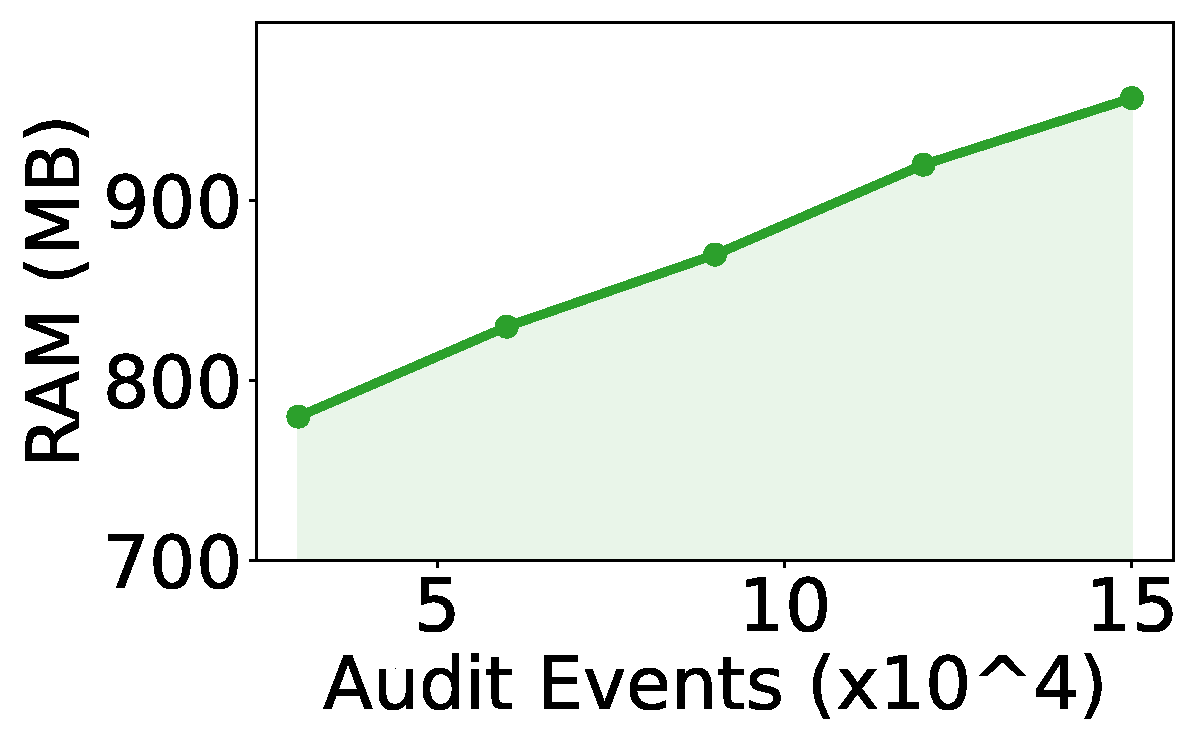
\includegraphics[width=0.20\textwidth]{fig/ram.pdf}\label{ram_client}}
  \hfill
  \subfloat[CPU utilization central server.]{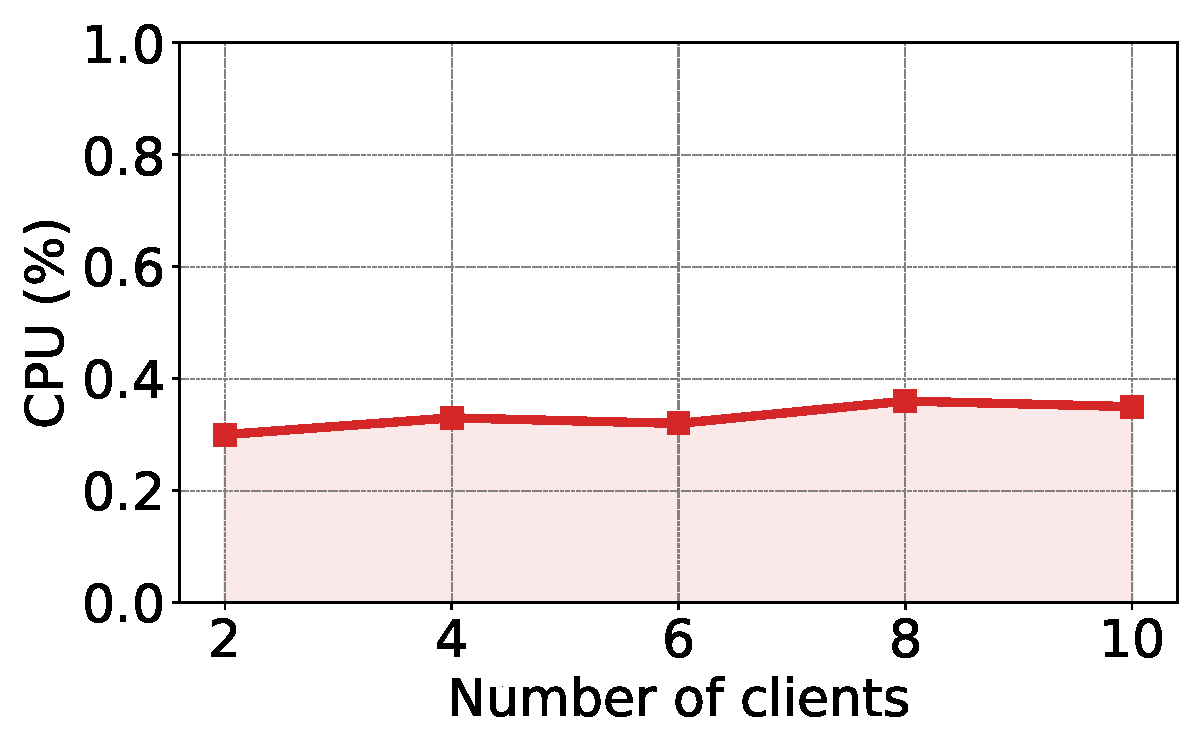
\includegraphics[width=0.20\textwidth]{fig/cpu_central.pdf}\label{cpu_central}}
  \hfill
  \subfloat[RAM utilization central server]{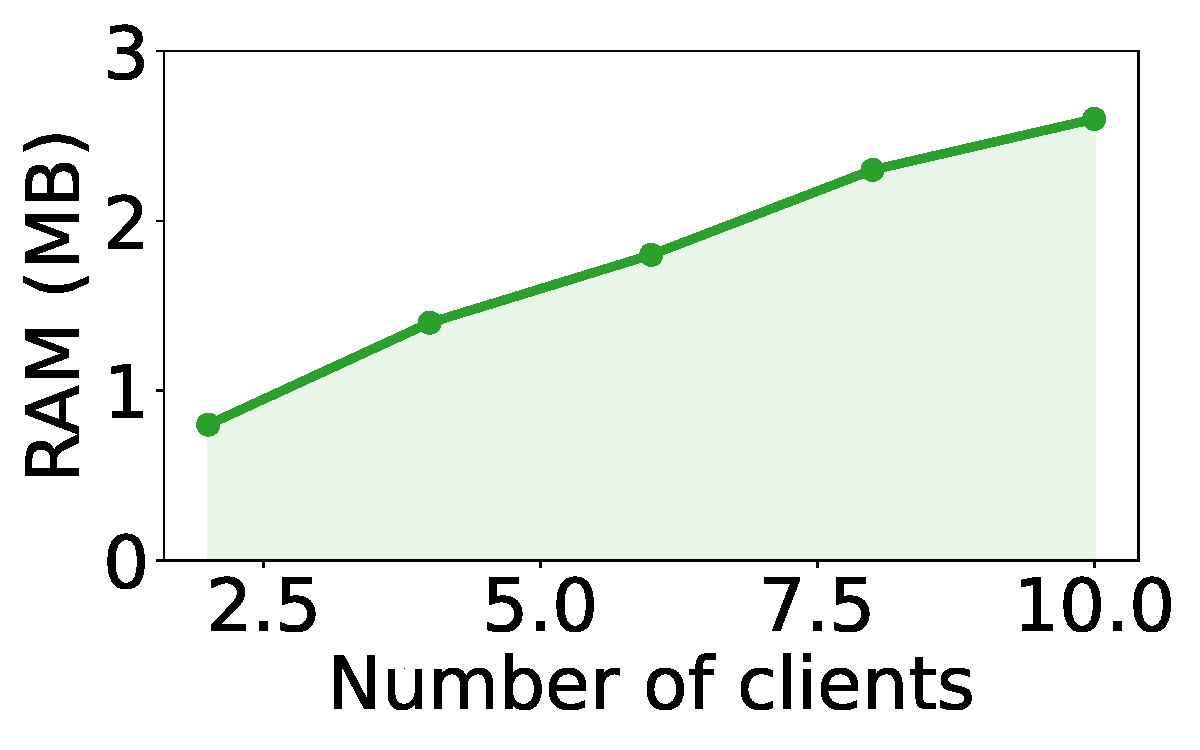
\includegraphics[width=0.20\textwidth]{fig/ram_central.pdf}\label{ram_central}}
  \hfill
  \subfloat[CPU utilization utility server.]{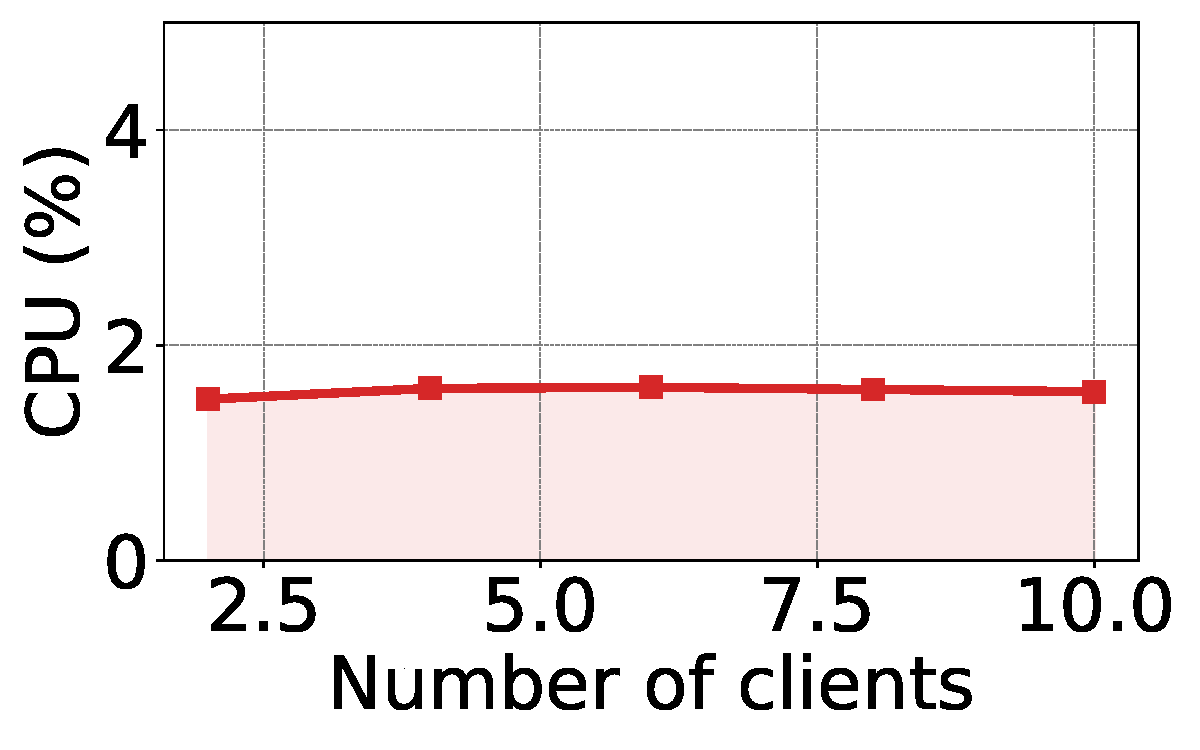
\includegraphics[width=0.20\textwidth]{fig/cpu_utility.pdf}\label{cpu_utility}}
  \hfill
  \subfloat[RAM utilization utility server]{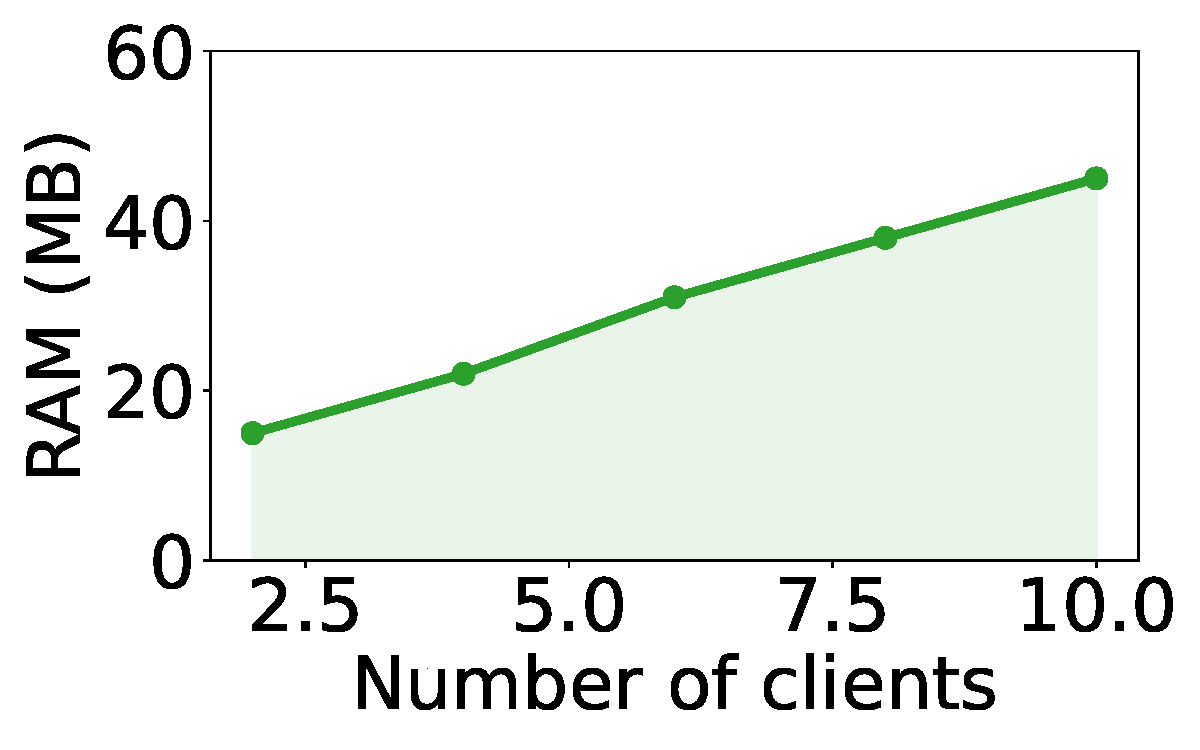
\includegraphics[width=0.20\textwidth]{fig/ram_utility.pdf}\label{ram_utility}}
  \caption{Resource consumption of various components of \Sys.}
  \label{fig:resource}
  \vspace{-2ex}
\end{figure}

 \subsection{Processing time analysis}

 We conducted experiments to study the end-to-end processing time of our system for a client machine. For this, we used batches of audit events of various sizes, conducting end-to-end inference with \Sys to measure the time taken to process these events on a client machine. The results, illustrated in Figure~\ref{sizevstime}, demonstrate that \Sys processes events with notable efficiency. For example, it requires approximately 23 seconds to process a batch of 100,000 events. Given our previous analysis of host logs in the \optc dataset, which indicated that each host generates an average of 100,000 events in three hours, \Sys can process 24 hours worth of log data on a client in merely 3 minutes. This level of efficiency ensures that our system is highly effective, preventing any potential log congestion.

 \begin{figure}[!t]
  \centering
  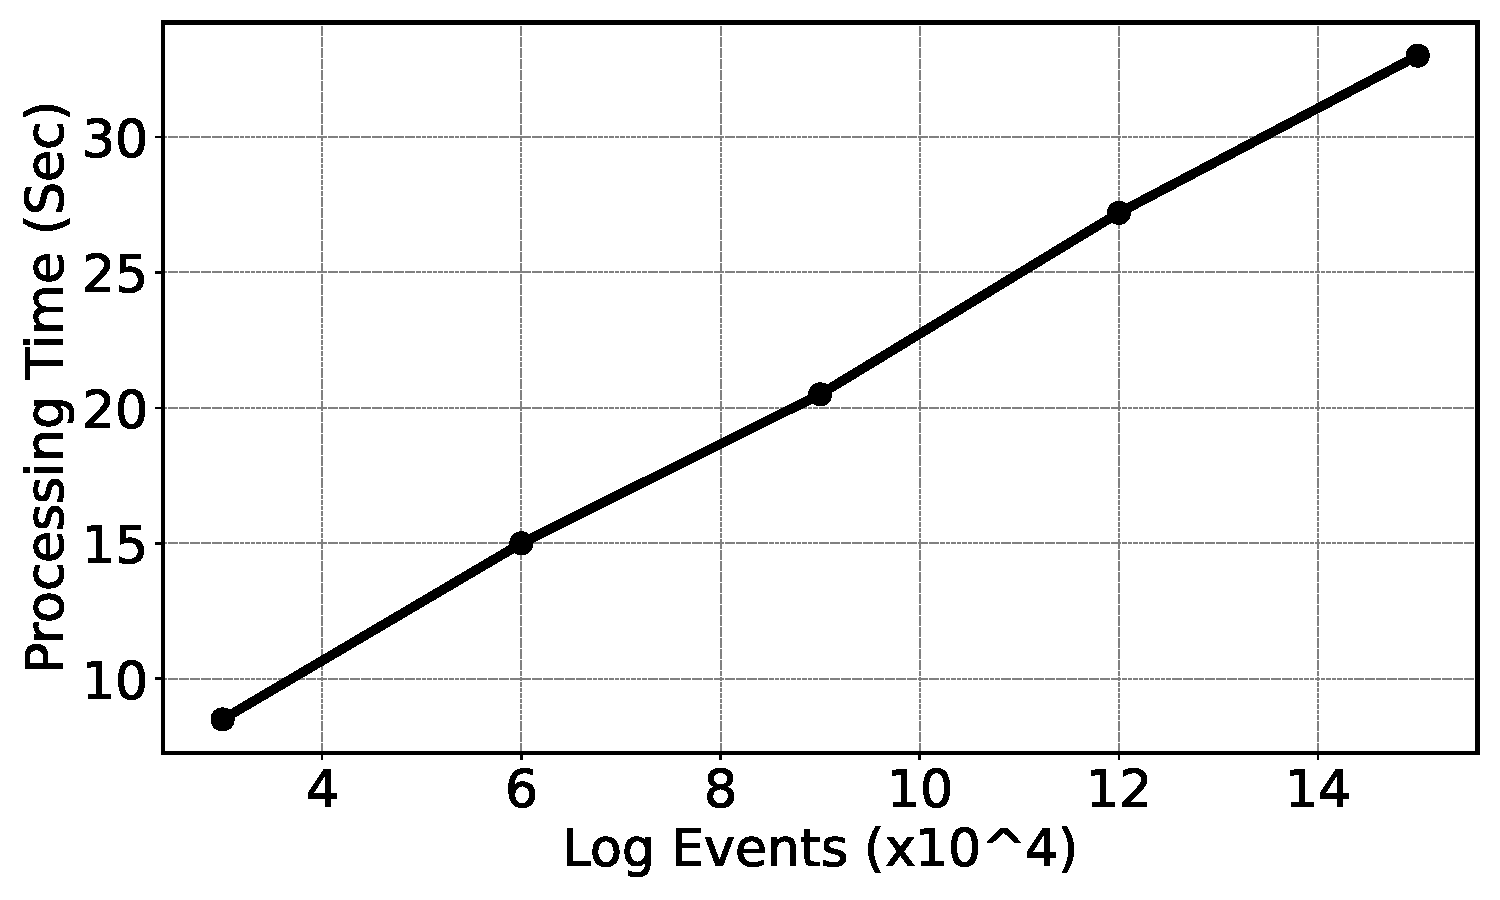
\includegraphics[width=0.25\textwidth]{fig/sizevstime.pdf}
  \caption{Processing time for various audit event sizes evaluated using \optc dataset.}
  \label{sizevstime}
  \vspace{-2ex}
\end{figure}

\subsection{Cost metric analysis}
\label{cost_metric}
We examined the operational costs of deploying \Sys in comparison to centralized solutions like \flash and \kairos for organizational use. Our evaluation concentrates on three primary cost components: network expenses (\(C_{N}\)), the cost of storing raw data (\(C_{S}\)), and processing costs (\(C_{P}\)).

To begin, we estimate these costs for the \flash system utilizing the \optc dataset. Each host within \optc produces approximately 1GB of audit logs daily, equating to nearly one million audit events. For an organization with 1,000 hosts, the total daily log volume would be 1,000 GB. This data volume requires transmission over the network and storage on a central server operating \flash. Additionally, \flash processes one million events in about 100 seconds, implying that processing events from 1,000 clients would necessitate approximately 27.7 hours. In contrast, \kairos processes 57,000 events in 11.6 seconds, leading to a processing time of 204 seconds for one million events. Consequently, processing data from 1,000 clients with \kairos would require around 56.6 hours.

To calculate the daily operational costs of running these systems for a specific organization, we utilized the Google Cloud Platform's (GCP) pricing calculator~\cite{gcp}. The cost to operate \flash under the previously mentioned workload is estimated at \$135, with computing expenses accounting for \$100 and storage and network costs comprising \$35. Given its longer processing duration, the operational cost for \kairos would be twice that of \flash.

Compared to existing systems, \Sys processes client logs in a federated manner, eliminating the need for logs to leave the client's machine. The only network expenses arise from the transmission of \gnnshort and Word2Vec models. Specifically, the \gnnshort model is 13kb, while the average Word2Vec model is 6 MB. For an organization with 1,000 hosts, the communication cost with the central server would be 12.70 MB, and for the utility server, it would be 5.86 GB. Overall, \Sys achieves a 170-fold reduction in communication and centralized storage costs compared to \flash and \kairos. The central and utility servers conduct a simple mean operation on the models, taking only a few seconds. Therefore, the operational cost of \Sys for 1,000 client machines is approximately \$10 per day, marking a 13-fold reduction compared to \flash and a 26-fold reduction compared to \kairos.

\subsection{Effect of differential privacy on accuracy}

Differential privacy is a method that can be combined with federated learning to offer protection against inference attacks~\cite{lyu2020threats,nasr2019comprehensive,zari2021efficient} at the cost of detection accuracy. We have analyzed the robustness of our system against these attacks in Section~\ref{privacy}. Here we will examine the impact of differential privacy noise levels on the detection performance of \Sys. Differential privacy is a method designed to ensure the privacy and confidentiality of the data points when used in machine learning models. It achieves this by adding a controlled amount of random noise to the model parameters, which helps in concealing the influence of any individual data point. In our context, differential privacy introduces a parameter called epsilon $\epsilon$ which dictates the intensity of noise added to the local \gnnshort model updates before they are aggregated at the central server for federated averaging, as detailed in Section~\ref{sec:methodology}.

The parameter $\epsilon$ is crucial; it is inversely related to the amount of noise added -- lower values of $\epsilon$ result in higher noise levels, thereby increasing privacy but potentially degrading the utility of the model. Conversely, a higher $\epsilon$ indicates less noise, which may improve the model's detection capabilities but reduce privacy protection. By adjusting $\epsilon$ during the training phase, we assess the trade-off between privacy and detection performance in the globally trained models across various $\epsilon$ settings. Figure~\ref{epsvsscore} shows that increasing noise strength degrades model utility offering more privacy at the expense of reduced accuracy.

\begin{figure}[!t]
  \centering
  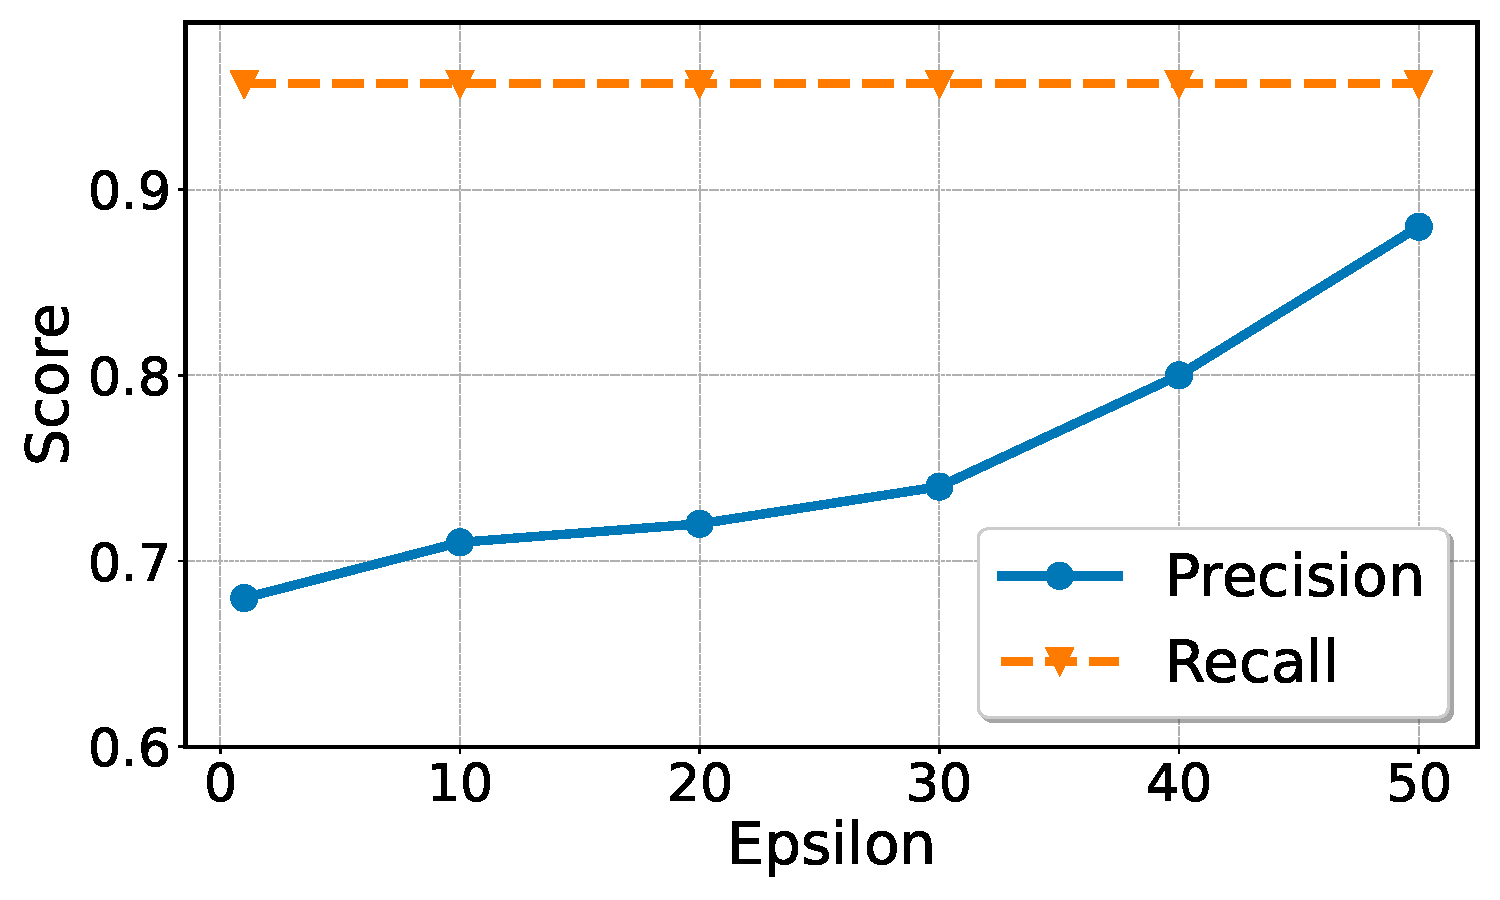
\includegraphics[width=0.25\textwidth]{fig/epsvsscore.pdf}
  \caption{Effect of differential privacy noise on detection using E3 dataset. Note that we observed similar results on the other datasets.}
  \label{epsvsscore}
  \vspace{-2ex}
\end{figure}


% \begin{figure*}[!t]
%   \centering
%   \subfloat[Anomaly threshold effect.]{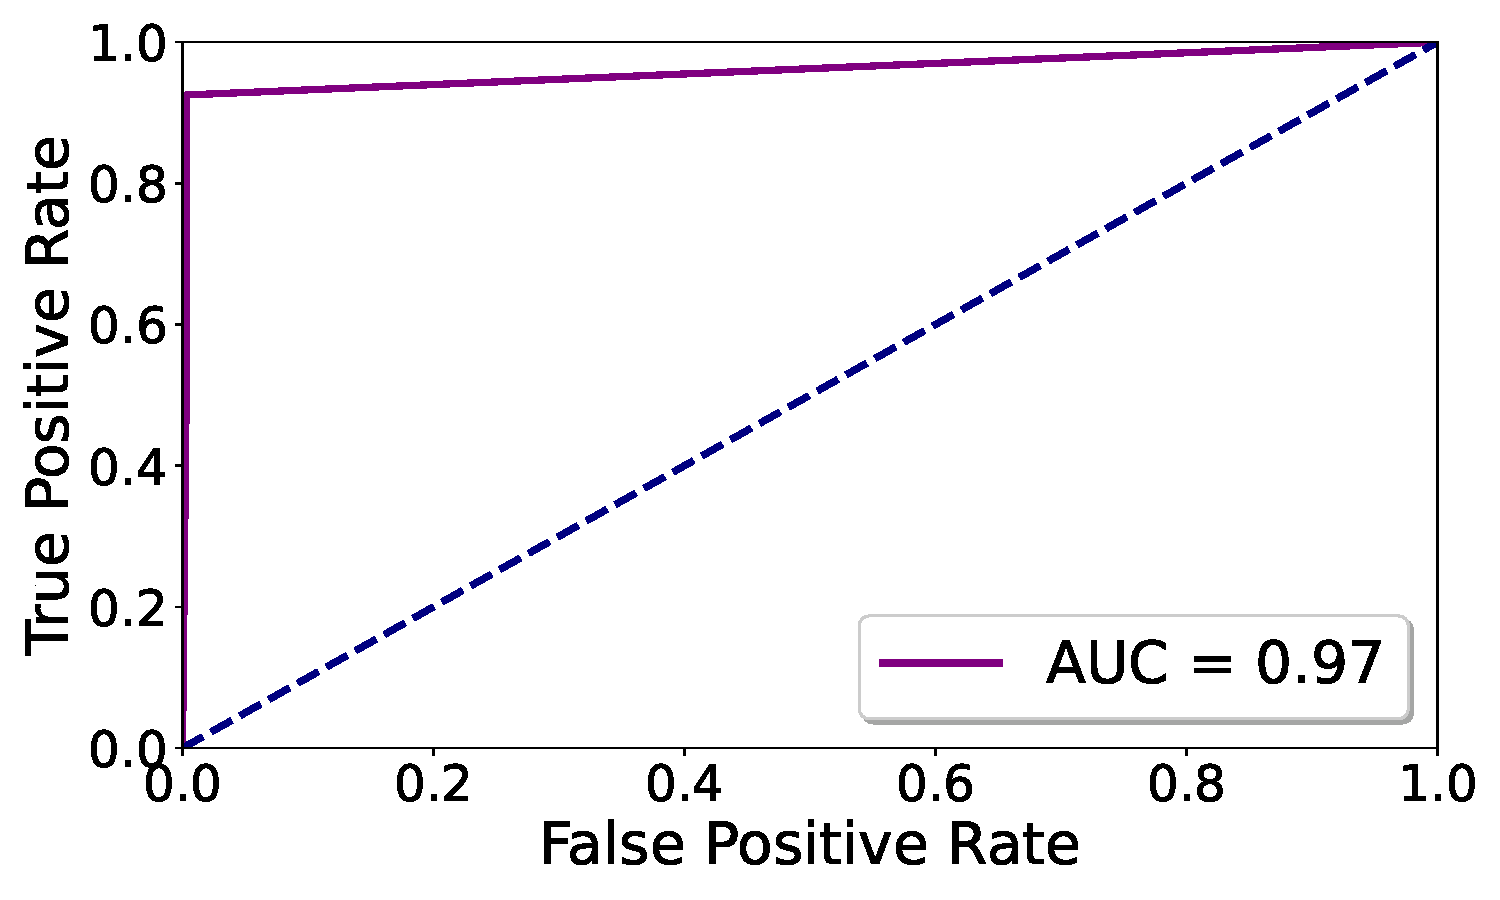
\includegraphics[width=0.24\textwidth]{fig/thresh.pdf}\label{thresh}}
%   \hfill
%   \subfloat[Effect of number of categories vs detection performance using E3 dataset.]{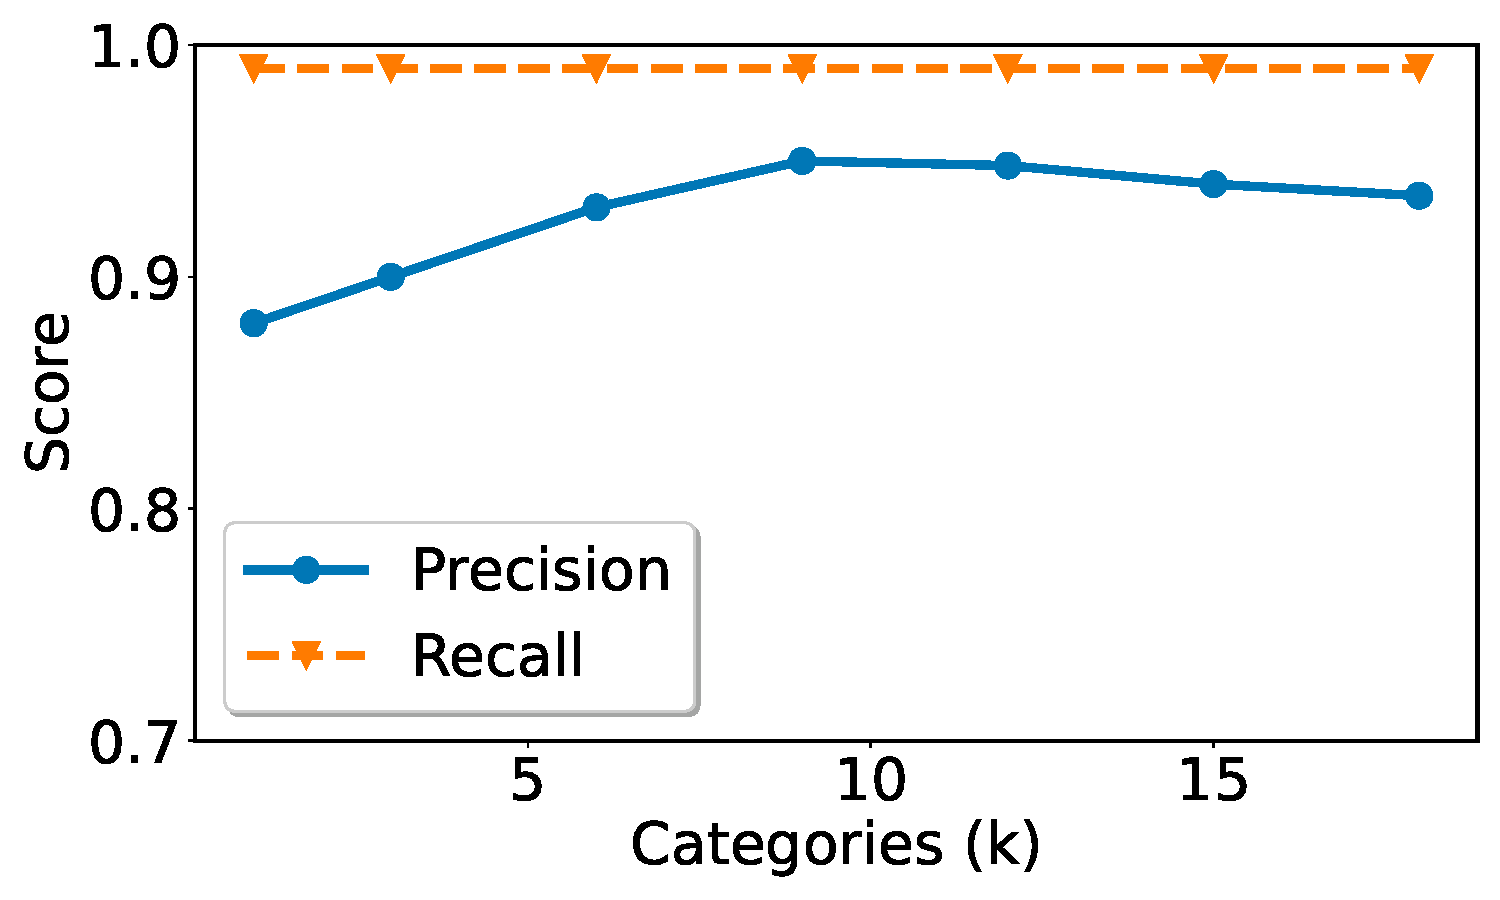
\includegraphics[width=0.24\textwidth]{fig/kvsscore.pdf}\label{catgvsscore}}
%   \hfill
%   \subfloat[Federated averaging rounds vs detection performance using E3 dataset.]{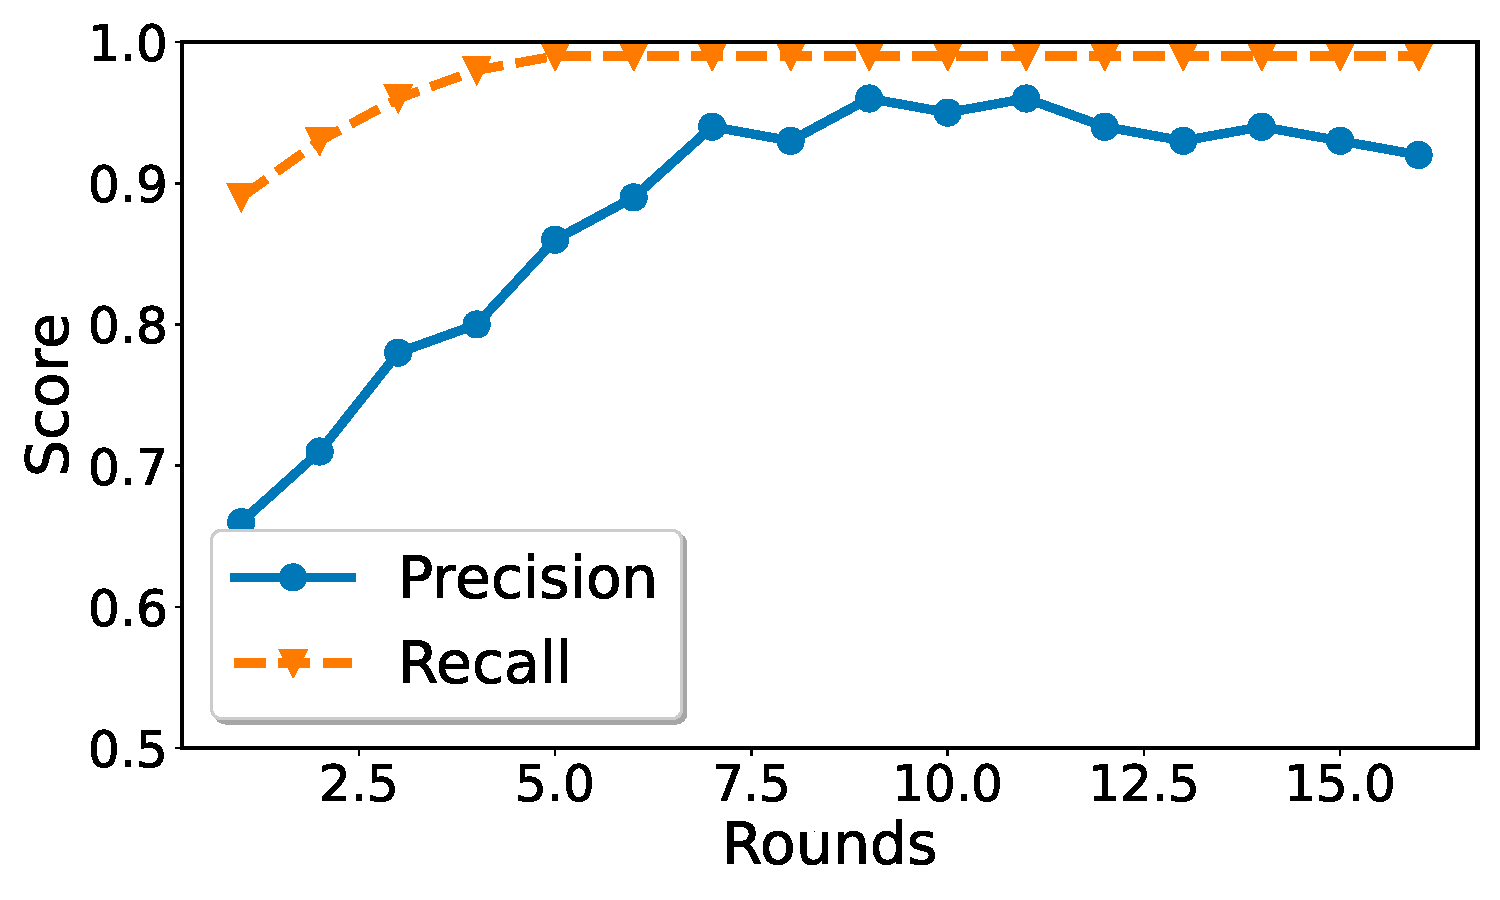
\includegraphics[width=0.24\textwidth]{fig/roundsvsscore.pdf}\label{roundsvsscore}}
%   \hfill
%   \subfloat[Effect of number of hosts vs detection metrics using \optc dataset]{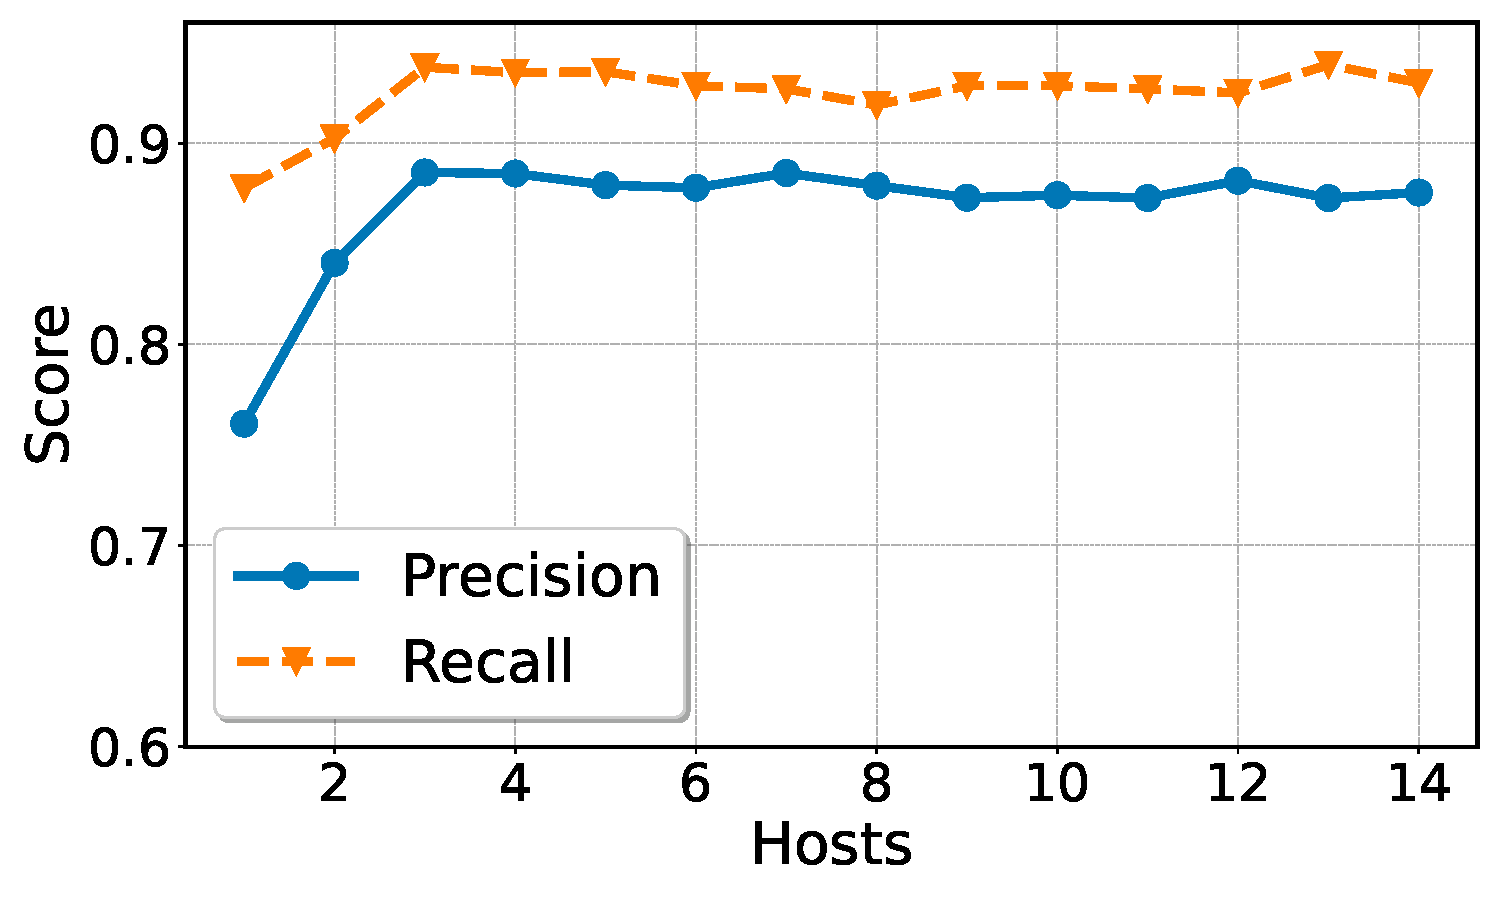
\includegraphics[width=0.24\textwidth]{fig/scoresvshosts.pdf}\label{rscoresvshosts}}
%   \caption{Ablation Study of various \Sys components.}
%   \label{ablation}
%   \vspace{-2ex}
% \end{figure*}
